%\documentclass[aps,prb,twocolumn,superscriptaddress,preprintnumbers,amsmath,amssymb,floatfix]{revtex4}
\documentclass[aps,prb,preprint,superscriptaddress,amsmath,amssymb,floatfix]{revtex4}
%\documentclass[aps,prl,onecolumn,groupedaddress,amsmath,amssymb,12pt]{revtex4}
\usepackage[dvips]{epsfig}
\usepackage{graphicx}
\usepackage{ifthen}
\usepackage{dcolumn}% Align table columns on decimal point
\usepackage{bm}% bold math
\usepackage{multirow}
\usepackage{booktabs}
\usepackage{bm}% bold math
\usepackage{amsbsy}
\usepackage{amsmath}
\usepackage{amssymb}
\usepackage{subfigure}
\usepackage{wrapfig}
\usepackage{hyperref}


%Definition of new commands
\newcommand{\f}[2]{\ensuremath{\frac{\displaystyle{#1}}{\displaystyle{#2}}}}
\newcommand{\lr}[1]{\langle{#1}\rangle}
\newcommand{\colv}[2] {\left(\begin{array}{c} #1 \\ #2 \end{array}\right)}
\renewcommand{\thefootnote}{\fnsymbol{footnote}}
\newcommand{\be} {\begin{eqnarray}}
\newcommand{\ee} {\end{eqnarray}}
%--------------------------------------------------------------------------
%EQ COMMANDS
%--------------------------------------------------------------------------
\newcommand{\two}{\mspace{-2.0mu}}
\newcommand{\four}{\mspace{-4.0mu}}
\newcommand{\plus}{\mspace{-4.5mu}+\mspace{-3.5mu}}
\newcommand{\minus}{\mspace{-4.5mu}-\mspace{-3.5mu}}
\newcommand{\pp}{'\mspace{-2.0mu}'}
\newcommand{\xlb}[4]{#1\ifthenelse{\equal{#2}{0}}{}{_{\alpha #2}}
\mspace{-2.0mu}\genfrac{(}{)}{0pt}{1}{\ifthenelse{\equal{#3}{0}}{0}{l #3}} 
{\ifthenelse{\equal{#4}{0}}{0}{b #4}}}

\newcommand{\xkv}[4]{#1\mspace{-5.0mu}\left(\mspace{-8.0mu}
\begin{smallmatrix}#2\four{}\four{}\mspace{-8.0mu}&\pmb{\kappa}#3\\&\nu 
#4\end{smallmatrix}\mspace{-5.0mu}\right)}

\newcommand{\evect}[6]{#1\mspace{-4.0mu}\left(\mspace{-8.0mu}
\begin{smallmatrix}#2\mspace{-8.0mu}&\pmb{\kappa} #3 &b #5\\&\nu #4 &
\alpha #6\end{smallmatrix}\mspace{-5.0mu}\right)}

\newcommand{\varmat}[8]{\mspace{-5.0mu}\left(\mspace{-8.0mu}
\begin{smallmatrix}\ifthenelse{\equal{#3}{0}}{\mspace{-8.0mu}&b_{#1}&b_{#2}
\\&\alpha_{#1}&\alpha_{#2}} {\ifthenelse{\equal{#7}{0}}{#1\mspace{-8.0mu}&
\pmb{\kappa}#2#3\mspace{-8.0mu}&\pmb{\kappa}#4#5\mspace{-8.0mu}&\pmb{\kappa}
#6\\&\nu#2&\nu#4&\nu#6} {#1\mspace{-8.0mu}&\pmb{\kappa}#2#3\mspace{-8.0mu}&
\pmb{\kappa}#4#5\mspace{-8.0mu}&\pmb{\kappa}#6#7\mspace{-8.0mu}&\pmb{\kappa}
#8\\&\nu#2&\nu#4&\nu#6&\nu#8}}\end{smallmatrix}\mspace{-5.0mu}\right)}

\newcommand{\EXP}[1]{\exp\mspace{-5.0mu}\left[#1\right]\mspace{-3.0mu}}

\newcommand{\tpp}[2]{\left(\mspace{-2.0mu}\xkv{\omega}{}{}{}#1\xkv{\omega}
{}{'}{'}#2\xkv{\omega}{}{\pp}{\pp}\mspace{-2.0mu}\right)}



%--------------------------------------------------------------------------
\newcommand{\SUM}[2]{\ifthenelse{\equal{#1}{0}}{\sum_{
\alpha_{#2},b_{#2},l_{#2}}^{3,n,N}} {\ifthenelse{\equal{#1}{1}}{\sum_{
\alpha_{#2},b_{#2}}^{3,n}}{\sum_{\pmb{\kappa}#2,\nu#2}^{N,3n}}}}

\newcommand{\SUMprime}[2]{\ifthenelse{\equal{#1}{0}}
{\sum_{\alpha_{#2},b_{#2},l_{#2}}^{3,n,N}} 
{\ifthenelse{\equal{#1}{1}}{\sum_{\alpha_{#2},b_{#2}}^{3,n}}
{\sum_{\pmb{\kappa}^{'}#2,\nu#2}^{N,3n}}}}

\newcommand{\SUMalpha}[2]{\ifthenelse{\equal{#1}{0}}
{\sum_{\alpha_{#2}}^{3}} {\ifthenelse{\equal{#1}{1}}
{\sum_{\alpha_{#2},b_{#2}}^{3,n}}{\sum_{\pmb{\kappa}#2,\nu#2}^{N,3n}}}}
%--------------------------------------------------------------------------
\newcommand{\SUMalphap}[2]{\ifthenelse{\equal{#1}{0}}
{\sum_{\alpha'_{#2}}^{3}} {\ifthenelse{\equal{#1}{1}}
{\sum_{\alpha'_{#2},b'_{#2}}^{3,n}}{\sum_{\pmb{\kappa}#2,\nu#2}^{N,3n}}}}

\newcommand{\SUMb}[2]{\ifthenelse{\equal{#1}{0}}{\sum_{b_{#2}}^{n}}
 {\ifthenelse{\equal{#1}{1}}{\sum_{\alpha_{#2},b_{#2}}^{3,n}}
{\sum_{\pmb{\kappa}#2,\nu#2}^{N,3n}}}}

\newcommand{\SUMbp}[2]{\ifthenelse{\equal{#1}{0}}{\sum_{b'_{#2}}^{n}}
 {\ifthenelse{\equal{#1}{1}}{\sum_{\alpha'_{#2},b'_{#2}}^{3,n}}
{\sum_{\pmb{\kappa}#2,\nu#2}^{N,3n}}}}

\newcommand{\SUMl}[2]{\ifthenelse{\equal{#1}{0}}{\sum_{l_{#2}}^{N}}
 {\ifthenelse{\equal{#1}{1}}{\sum_{\alpha_{#2},b_{#2}}^{3,n}}
{\sum_{\pmb{\kappa}#2,\nu#2}^{N,3n}}}}

\newcommand{\SUMlp}[2]{\ifthenelse{\equal{#1}{0}}{\sum_{l'_{#2}}^{N}}
 {\ifthenelse{\equal{#1}{1}}{\sum_{\alpha'_{#2},b'_{#2}}^{3,n}}
{\sum_{\pmb{\kappa}#2,\nu#2}^{N,3n}}}}

\newcommand{\abcdt}[5]{\mspace{-4.0mu}\left(\mspace{-8.0mu}
\begin{smallmatrix}&\ifthenelse{\equal{#1}{}}{a}{#1}&\ifthenelse
{\equal{#3}{}}{c}{#3}\\&\ifthenelse{\equal{#2}{}}{b}{#2}&\ifthenelse
{\equal{#4}{}}{d}{#4}\end{smallmatrix}\mspace{-2.0mu};\ifthenelse
{\equal{#5}{}}{t}{#5}\right)}

\newcommand{\abcd}[4]{\mspace{-4.0mu}\left(\mspace{-8.0mu}
\begin{smallmatrix}&\ifthenelse{\equal{#1}{}}{a}{#1}&\ifthenelse
{\equal{#3}{}}{c}{#3}\\&\ifthenelse{\equal{#2}{}}{b}{#2}&\ifthenelse
{\equal{#4}{}}{d}{#4}\end{smallmatrix}\mspace{-3.0mu}\right)}

\newcommand{\abt}[3]{\mspace{-4.0mu}\left(\mspace{-8.0mu}\begin
{smallmatrix}&\ifthenelse{\equal{#1}{}}{a}{#1} \\&\ifthenelse{
\equal{#2}{}}{b}{#2}\end{smallmatrix}\mspace{-2.0mu};
\ifthenelse{\equal{#3}{}}{t}{#3}\right)}

\newcommand{\ab}[2]{\mspace{-4.0mu}\left(\mspace{-8.0mu}
\begin{smallmatrix}&\ifthenelse{\equal{#1}{}}{a}{#1} \\&\ifthenelse
{\equal{#2}{}}{b}{#2}\end{smallmatrix}\mspace{-3.0mu}\right)}

\newcommand{\kvbat}{\mspace{-4.0mu}\left(\mspace{-8.0mu}
\begin{smallmatrix} &\pmb{\kappa} &b \\ &\nu &\alpha\end{smallmatrix}
\mspace{-2.0mu};t\right)}
%--------------------------------------------------------------------------
\newcommand{\kvbatp}{\mspace{-4.0mu}\left(\mspace{-8.0mu}
\begin{smallmatrix} &\pmb{\kappa} &b' \\ &\nu &\alpha'\end{smallmatrix}
\mspace{-2.0mu};t\right)}

\newcommand{\kvbaw}{\mspace{-4.0mu}\left(\mspace{-8.0mu}
\begin{smallmatrix} &\pmb{\kappa} &b \\ &\nu &\alpha\end{smallmatrix}
\mspace{-2.0mu};\omega\right)}

\newcommand{\kvbawp}{\mspace{-4.0mu}\left(\mspace{-8.0mu}
\begin{smallmatrix} &\pmb{\kappa} &b' \\ &\nu &\alpha'\end{smallmatrix}
\mspace{-2.0mu};\omega\right)}

\newcommand{\kvba}{\mspace{-4.0mu}\left(\mspace{-8.0mu}
\begin{smallmatrix} &\pmb{\kappa} &b \\ &\nu &\alpha\end{smallmatrix}
\mspace{-3.0mu}\right)}

\newcommand{\kvbap}{\mspace{-4.0mu}\left(\mspace{-8.0mu}
\begin{smallmatrix} &\pmb{\kappa} &b' \\ &\nu &\alpha'\end{smallmatrix}
\mspace{-3.0mu}\right)}
%--------------------------------------------------------------------------
\newcommand{\kpvba}{\mspace{-4.0mu}\left(\mspace{-8.0mu}
\begin{smallmatrix} &\pmb{\kappa}^{'} &b \\ &\nu &\alpha\end{smallmatrix}
\mspace{-3.0mu}\right)}

\newcommand{\kva}{\mspace{-4.0mu}\left(\mspace{-8.0mu}
\begin{smallmatrix} &\pmb{\kappa} \\ &\nu &\alpha\end{smallmatrix}
\mspace{-3.0mu}\right)}

\newcommand{\kvap}{\mspace{-4.0mu}\left(\mspace{-8.0mu}
\begin{smallmatrix} &\pmb{\kappa} \\ &\nu &\alpha'\end{smallmatrix}
\mspace{-3.0mu}\right)}

\newcommand{\kvb}{\mspace{-4.0mu}\left(\mspace{-8.0mu}
\begin{smallmatrix} &\pmb{\kappa} &b \\ &\nu \end{smallmatrix}
\mspace{-3.0mu}\right)}

\newcommand{\kvbp}{\mspace{-4.0mu}\left(\mspace{-8.0mu}
\begin{smallmatrix} &\pmb{\kappa} &b' \\ &\nu \end{smallmatrix}
\mspace{-3.0mu}\right)}

\newcommand{\kvt}{\mspace{-4.0mu}\left(\mspace{-8.0mu}
\begin{smallmatrix}&\pmb{\kappa} \\&\nu\end{smallmatrix}
\mspace{-2.0mu};t\right)}

\newcommand{\kpvt}{\mspace{-4.0mu}\left(\mspace{-8.0mu}
\begin{smallmatrix}&\pmb{\kappa}^{'} \\&\nu\end{smallmatrix}
\mspace{-2.0mu};t\right)}

\newcommand{\kvw}{\mspace{-4.0mu}\left(\mspace{-8.0mu}
\begin{smallmatrix}&\pmb{\kappa} \\&\nu\end{smallmatrix}
\mspace{-2.0mu};\omega\right)}

\newcommand{\kv}{\mspace{-4.0mu}\left(\mspace{-8.0mu}
\begin{smallmatrix}&\pmb{\kappa} \\&\nu\end{smallmatrix}
\mspace{-3.0mu}\right)}

\newcommand{\kpvp}{\mspace{-4.0mu}\left(\mspace{-8.0mu}
\begin{smallmatrix}&\pmb{\kappa'} \\&\nu'\end{smallmatrix}
\mspace{-3.0mu}\right)}
%--------------------------------------------------------------------------
\newcommand{\lbt}{\mspace{-4.0mu}\left(\mspace{-8.0mu}
\begin{smallmatrix}&l \\&b\end{smallmatrix}\mspace{-2.0mu};t\right)}

\newcommand{\lbtp}{\mspace{-4.0mu}\left(\mspace{-8.0mu}
\begin{smallmatrix}&l' \\&b'\end{smallmatrix}\mspace{-2.0mu};t\right)}

\newcommand{\lt}{\mspace{-4.0mu}\left(\mspace{-8.0mu}
\begin{smallmatrix}&l\end{smallmatrix}\mspace{-2.0mu};t\right)}

\newcommand{\ltp}{\mspace{-4.0mu}\left(\mspace{-8.0mu}
\begin{smallmatrix}&l'\end{smallmatrix}\mspace{-2.0mu};t\right)}

\newcommand{\lb}{\mspace{-4.0mu}\left(\mspace{-8.0mu}
\begin{smallmatrix}&l \\&b\end{smallmatrix}\mspace{-3.0mu}\right)}

\newcommand{\lbp}{\mspace{-4.0mu}\left(\mspace{-8.0mu}
\begin{smallmatrix}&l' \\&b'\end{smallmatrix}\mspace{-3.0mu}\right)}
%--------------------------------------------------------------------------
%COMMANDS
%--------------------------------------------------------------------------
\begin{document}
%--------------------------------------------------------------------------
\title{Predicting Vibrational Mean Free Paths in Disordered Systems}
%--------------------------------------------------------------------------
\author{Jason M. Larkin}
\affiliation{Department of Mechanical Engineering\\Carnegie Mellon 
University\\Pittsburgh, PA 15213}
\author{A. J. H. McGaughey}
\email{mcgaughey@cmu.edu}
\affiliation{Department of Mechanical Engineering\\
Carnegie Mellon University\\Pittsburgh, PA 15213}
%--------------------------------------------------------------------------
\date{\today}
%--------------------------------------------------------------------------
\begin{abstract}
Understanding thermal transport in crystalline systems requires detailed 
knowledge of phonons, which are the quanta of energy associated with atomic 
vibrations. By definition, phonons are non-localized vibrations that 
transport energy over distances much larger than the atomic spacing. For 
disordered materials (e.g., alloys, amorphous phases), with the exception 
of very long wavelength modes, the vibrational modes are localized and do 
not propagate like phonons. The Einstein model assumes that the mean free 
path of these localized vibrations is the average interatomic distance and 
that their group velocity is equal to the speed of sound. The Cahill-Pohl 
model assumes that the mean free path of the localized modes is equal to 
half of their wavelength. While these approach can be used to estimate the 
thermal conductivity of disordered systems, they only 
provide a qualitative description of the vibrations that contribute to the 
lattice thermal conductivity.
Using lattice dynamics calculations and molecular dynamics simulations on 
Lennard-Jones crystalline, alloy, and amorphous systems, we predict and 
characterize the contributions from phonons and localized vibrations to 
lattice thermal conductivity. 

% The results are used to motivate simple and 
% computationally cheap models to predict the lattice thermal conductivity 
% of a range of disordered materials.
\end{abstract}
%--------------------------------------------------------------------------
\maketitle
%--------------------------------------------------------------------------
\clearpage
\section{\label{S:Introduction}Introduction}
%--------------------------------------------------------------------------
The thermal conductivity of amorphous solids display 
unique temperature dependance compared to ordered solids.
\cite{freeman_thermal_1986} 
Cahill argued that the lattice vibrations 
in a disordered crystal are essentially the same as those of an amorhous 
solid.
\cite{cahill_lower_1992} 

Measurements by all the refs from Galli paper, including Moon.
\cite{wada_thermal_1996,zink_thermal_2006,yang_anomalously_2010,
cahill_thermal_1994,kuo_thermal_1992,moon_thermal_2002,liu_high_2009}
The key to understanding such measurement is to estimate a MFP for the 
vibrational modes in disordered systems. 

The goal of this work is to predict the MFP of vibrational modes in 
disordered systems. Simple Lennard-Jones systems will be studied.  A 
perfect LJ crystal are alloyed with a species of differing mass and 
amorphous samples are prepared. Thermal transport will be studied to 
quantify and characterize the ordered and 
disordered contributions to lattice thermal conductivity. In particular, a 
more rigorous way to classify vibrational modes in disordered alloys and 
amorphous samples as phonon-like or diffuson will be investigated. These 
results will be compared to the phenomenological Einstein and Cahill-Pohl 
models,\cite{einstein1911,kittel1949,cahill1992}.

The vibrational modes in these systems are
characterized in the limit of propagating (phonon) and 
non-propagating (diffuson) modes by predicting the mode lifetimes and 
estimating their mean free paths. Estimating an effective dispersion
relation is necessary for calculating an effective group velocity for 
disordered, which is crucial for transforming lifetimes to MFPs.
The spectrum of phonon MFPs and the accumulated thermal conductivity 
are predicted for a model of amorphous silicon. Predictions of thermal 
conductivity using a boundary scattering model demonstrates  
%--------------------------------------------------------------------------
\section{\label{S:Lifetimes}Thermal Conductivity Predictions from 
Molecular Dynamics}
%--------------------------------------------------------------------------
The thermal conductivity of amorphous solids at low temperatures contain 
quantum statistical effects.\cite{freeman_thermal_1986} Molecular dynamics 
simulations are not able to capture quantum statistical effects.
%--------------------------------------------------------------------------
\begin{figure}
\begin{center}
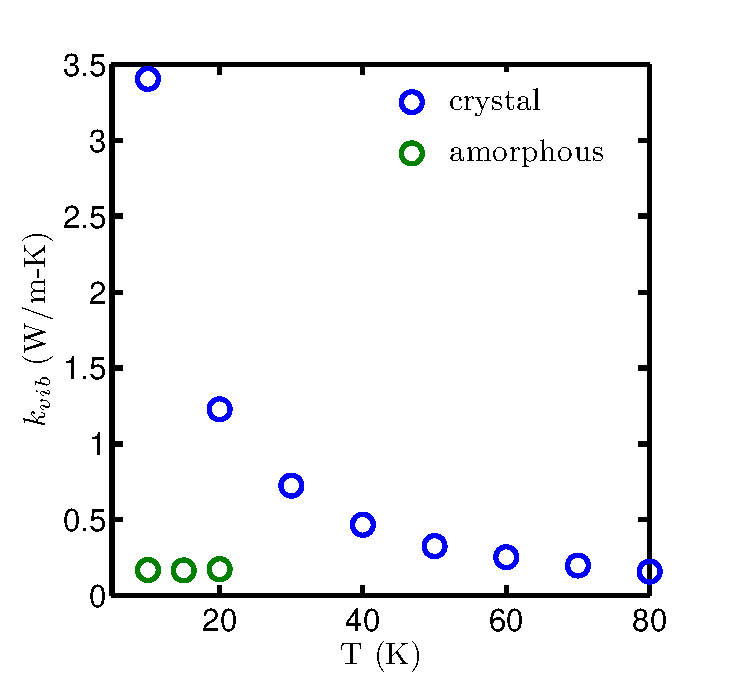
\includegraphics[scale=0.5]{LJ_amor_GK.eps}
\vspace*{-5mm}
\end{center}
\caption{\label{FIG:LJ_amor_GK}The temperature dependence of crystalline 
and amorphous Lennard-Jones samples predicted using MD simulations and the 
Green-Kubo method.\cite{mcgaughey2004a} For the crystal the vibrational 
conductivity follows a $1/T$ scaling (consistent with the phonon-phonon 
lifetime scaling in Eq$.$ \eqref{EQ:M:tau_p-p}) , while the amorphous 
vibrational conductivity is temperature independent. Both of these trends 
are due to the lack quantum mechanical effects in the classical MD 
simulations. }
\end{figure}
%--------------------------------------------------------------------------
\vspace*{40mm}
%--------------------------------------------------------------------------
\section{\label{S:Lifetimes}Kinetic Theory}
%--------------------------------------------------------------------------
k = sum over modes

For a perfect system, all vibrational modes are phonons.  

\begin{equation}\label{EQ:M:k_mode}
\begin{split}
k_{vib,\mathbf{n}}=&\sum_{\pmb{\kappa}} \sum_\nu c_{ph}\kv 
\pmb{v}^{2}_{g,\mathbf{n}}\kv \tau\kv.
\end{split}
\end{equation}

Of particular interest if the phonon mean free path (MFP),

\begin{equation}\label{EQ:M:phonon_mfp}
\begin{split}
\Lambda\kv = |\pmb{v}_{g}| \tau\kv,
\end{split}
\end{equation}

which requires a group velocity.

%--------------------------------------------------------------------------
\subsection{\label{S:Lifetimes:}Cahill-Pohl Model}
%--------------------------------------------------------------------------
Einstein model:

The group velocity for all the modes is equal to the speed of sound and the 
mean free path is given by the average interatomic spacing.
\cite{kittel_interpretation_1949,cahill_lower_1992}

Cahill-Pohl (CP) model:

The group velocity for all the modes is equal to the speed of sound and 
the lifetime is given by the inverse of the mode frequency.
\cite{cahill_lower_1992}

(half the mode 
wave-length)

In the Cahill-Pohl model,
\cite{PhysRevB.46.6131} the group velocity of all the vibrational modes is 
assumed to be the sound speed,
\begin{equation}\label{E-Seq}
v_g = v_s \propto \sqrt{B_{glass}/\rho},
\end{equation}
and the phonon mean free paths scale with the wavelength of the mode,
\begin{equation}\label{EQ:M:l_glass}
\Lambda_{glass} = \lambda /2.
\end{equation}

This approach can be used to estimate a lower limit to the vibrational 
conductivity in amorphous and disordered systems.
\cite{cahill_lower_1992,cahill_thermal_1987} 
However, theory,\cite{allen_thermal_1993} experimental measurements,
\cite{graebner_phonon_1986} and simulation results
\cite{shenogin_predicting_2009} show that this approach can give only a 
qualitative description of the vibrations which contribute to the thermal 
conductivity in disordered systems.

%--------------------------------------------------------------------------
\section{\label{S:Lifetimes}Allen-Feldman Theory}
%--------------------------------------------------------------------------
The models for phonon scattering mechanisms described in Section 
\ref{S-Prelim-Phonon-Scattering} are successful for dilute alloys 
($c<0.1$).\cite{klemens1955,klemens1957} However, as the alloy 
concentration is increased, the vibrational modes become localized and 
non-propagating and a new description of the vibrational modes which 
carry the heat is required. For even more disordered systems, such as 
amorphous materials, the thermal transport is modeled using completely 
localized vibrations (called \emph{diffusons}) which propagate diffusively, 
as phonons do.\cite{allen1993} However, the propagation of these diffusons 
is (typically) much slower than the propagation of phonons which are able 
to carry heat over long distances before scattering. Thus, the vibrational 
conductivity of amorphous phase is typically several orders of magnitude 
less than crystalline phase.\cite{freeman1986,cahill1992}
The diffuson theory of Allen and Feldman is different than the 
phenomenological models discussed in Section \ref{S-Motivation-Amorphous} 
in that the only allowed wavevector is strictly $\mathbf{\kappa}= 0$ since 
the system is disordered. In reality, the vibrational conductivity has 
contributions from very-long wavelength phonon-like modes (see Section 
\ref{S-Prelim-Phonon-Scattering}). The disordered contribution to 
vibrational conductivity, $k_{AF}$, is given by
\begin{equation}\label{EQ:M:k_AF}
k_{AF} = \sum_i C(\omega_i) D_{AF}(\omega_i)
\end{equation}
where $C(\omega_i)$ and $D_{AF}(\omega_i)$ are the diffuson mode specific 
heat and diffusivity. The vibrational conductivity at low temperatures in 
disordered and amorphous materials is due to the low temperature behavior 
of the specific heat $C(\omega_i)$, which is dictated by Bose-Einstein 
statistics.\cite{allen1993} The theory of Allen and Feldman is purely 
harmonic. In the classical harmonic limit, $C(\omega_i) = k_{B}$ and 
$k_{AF}$ is temperature independent, which can be used to understand the 
amorphous LJ temperature independence of vibrational conductivity in Section 
\ref{S-Prelim-Vib-Cond-Ordered}.

Diffusons, locons and propagons \cite{allen_diffusons_1999}.

%--------------------------------------------------------------------------
\subsection{\label{S-Motivation}AF Diffusivity}
%--------------------------------------------------------------------------
Allen Feldman theory \cite{allen_thermal_1993}.

Feldman measure the DOS using the average level spacing.
\cite{feldman_numerical_1999} 

Predictions for a-Si, also effects of mass disorder.
\cite{feldman_thermal_1993}: is Di pinned near a value of Di~(1/3)va?

$D = 1/3 v_{s} a$

It was noticed by Birch and Clark (1940), and by Kit-
tel (1948) that in glasses κ(T ) at T >20K could be in-
terpreted as the specific heat C(T )/V multiplied by a
temperature-independent diffusivity D of order a2 ωD /3
where a is an interatomic distance. In the phonon-gas
model, this would correspond to l ≈ a, too small to jus-
tify use of the model. The success of this observation
implies that the dominant normal modes in a glass are of
the D variety, not P because P implies l ≫ a, and not L
because L implies D = 0 until anharmonic corrections are
added which make D depend on T . This successful (and
we believe, essentially correct) interpretation lost favor
after Anderson localization was understood, because a
misconception arose that the P/D boundary (which cer-
tainly lies low in the spectrum of a glass) should lie close
to the E/L boundary.

%--------------------------------------------------------------------------
\subsection{\label{S:Lifetimes:}Phonon Diffusivity}
%--------------------------------------------------------------------------
Taking the phonon mode specific heat to be $c_{ph} \kv = k_{B}$, the phonon 
mode specific vibrational conductivity (Eq$.$ \eqref{EQ:M:k_l,sum}) can be 
written as
\begin{equation}\label{EQ:k_sum}
\begin{split}
k_{vib,\mathbf{n}}=&\sum_{\pmb{\kappa}} \sum_\nu k_{B} D_{ph}\kv,
\end{split}
\end{equation}
and the vibrational conductivity is determined by the phonon mode 
diffusitivies, defined as
\begin{equation}\label{EQ:k_sum}
\begin{split}
D_{ph}\kv = v\kv^{2} \tau\kv.
\end{split}
\end{equation}
This concept is useful for understanding how the relevant phonon properties 
(lifetime and group velocity) affect the thermal transport. It is also useful 
for comparing the relative transport strength of diffusons and phonons. 
Fig. \ref{FIG:phonon_diff} plots the phonon and diffuson mode diffusivities 
of a 256 atom LJ crystal and amorphous system at T = 20 K. The number of 
vibrational modes is the same for these two systems, but the relative 
magnitudes of the diffusivities vary greatly. The phonons diffusivities are 
generally greater than the diffuson diffusivities. However, Brioullin zone 
boundary (see Section \ref{A-Allowed-Wavevectors-Ordered}) phonon modes have 
a finite lifetime but vanishing group velocities, giving $D_{ph}\kv = 0$.
\cite{dove1993} For crystalline systems with many atoms in the unit cell, 
the presence of optical phonon modes begins to trap heat in low-group velocity 
branches ($D_{ph}\kv \approx 0$, see Section \ref{S-Prelim-Phonon-Dispersion}), 
making the distinction between phonons and diffusons diffuclt. Based on their 
contribution to vibrational conductivity, these low diffusivity optical 
phonons are thermally indistinguishable from diffusons.
The parameters defining the phonon diffusivity (phonon lifetime and group 
velocity) are generally well-understood. In particular, design strategies 
to minimize both of these parameters exist (see Sections 
\ref{S-Prelim-Phonon-Scattering} and \ref{S-Prelim-Phonon-Dispersion} ). 
However, the design strategies to control the diffusons diffusivities 
($D_{AF}$) are not well understood.\cite{allen1993,shenogin2009} The diffuson 
theory does not consider the effects of anharmonicity, which cane be 
investigated using a combination of MD simulations and LD calculations.
\cite{shenogin2009}

%--------------------------------------------------------------------------
\begin{figure}
\begin{center}
\includegraphics[scale=0.6]
{/home/jason/thesis/proposal/paper/phonon_diff.eps}
\vspace*{-5mm}
\end{center}
\caption{\label{FIG:phonon_diff} plot comparison of phonon diffusivity 
versus AF mode diffusivity for a 256 atom LJ crystal and amorphous system. 
For both systems, the total number of vibrational modes is the same.}
\end{figure}
%--------------------------------------------------------------------------

%--------------------------------------------------------------------------
\section{\label{S-Prelim-Phonons-Amor}Phonons in Amorphous Materials }
%--------------------------------------------------------------------------
The diffuson theory is different than the phenomenological models 
discussed in Section \ref{S-Motivation-Amorphous} in that the only 
allowed wavevector is strictly $\mathbf{\kappa}= 0$ since the system is 
disordered. In reality, the vibrational conductivity has contributions 
from very-long wavelength phonon-like modes. Accordingly, the total 
vibrational conductivity in a disordered or amorphous system is the sum of 
contributions from diffusons and phonons,
\begin{equation}\label{EQ:M:k_thermal}
k_{vib} = k_{AF} + k_{ph}.
\end{equation}
Using the Green-Kubo method (see Section \ref{S-Prelim-Vib-Cond-Ordered}), 
the total vibrational conductivity of amorphous Lennard-Jones argon has 
been predicted to be $k_{l}=0.17$ W/m-K. The diffuson contribution is 
predicted to be $k_{AF} = 0.14$ W/m-K, which suggests 
$k_{ph} = 0.03$ W/m-K. Similar atomistic predictions have been made for 
amorphous silicon, where the phonon contribution was shown to be 
$k_{ph} = 0.5k_{vib}$.\cite{He2011a} However, the definition of the 
allowed wavevectors, and hence the phonon properties of the amorphous 
system, is not well understood.\cite{He2011a}
%--------------------------------------------------------------------------
\begin{figure}
\begin{center}
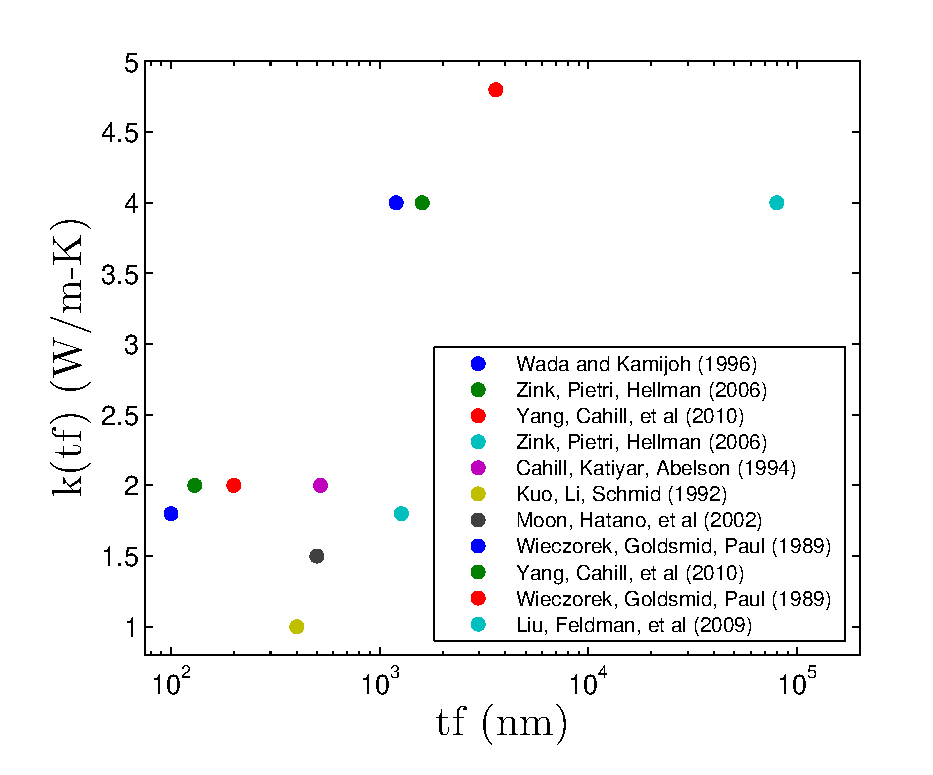
\includegraphics[scale=0.6]
{/home/jason/disorder/matlab/galli_si_k_tf.eps}
\vspace*{-5mm}
\end{center}
\caption{\label{FIG:phonon_diff} film thickness dependant thermal 
conductivity of a-Si from experiment.}
\end{figure}
%--------------------------------------------------------------------------

%--------------------------------------------------------------------------
\section{\label{S:Lifetimes}Lifetimes of Disordered Modes}
%--------------------------------------------------------------------------
Lifetimes in amorphous silicon predicted before using a normal mode 
approach, but mode-by-mode properties were not presented.
\cite{bickham_calculation_1998}

Lifetimes were predicted using anharmonic lattice dynamics, but no thermal 
transport properties were predicted.\cite{fabian_anharmonic_1996}

Thermal diffusivity was predicted for a percolation network which showed 
Rayleigh type scattering dependance in the low-frequency limit.
\cite{sheng_heat_1991}

Thermal diffusivity has been predicted using a wave-packet method

The lifetimes of vibrational modes in a-Si were predicted using normal 
mode decomposition.\cite{he_heat_2011}

%--------------------------------------------------------------------------
\subsection{\label{S:Lifetimes:}MFPs in Disordered Systems}
%--------------------------------------------------------------------------

%--------------------------------------------------------------------------
\begin{figure}
\begin{center}
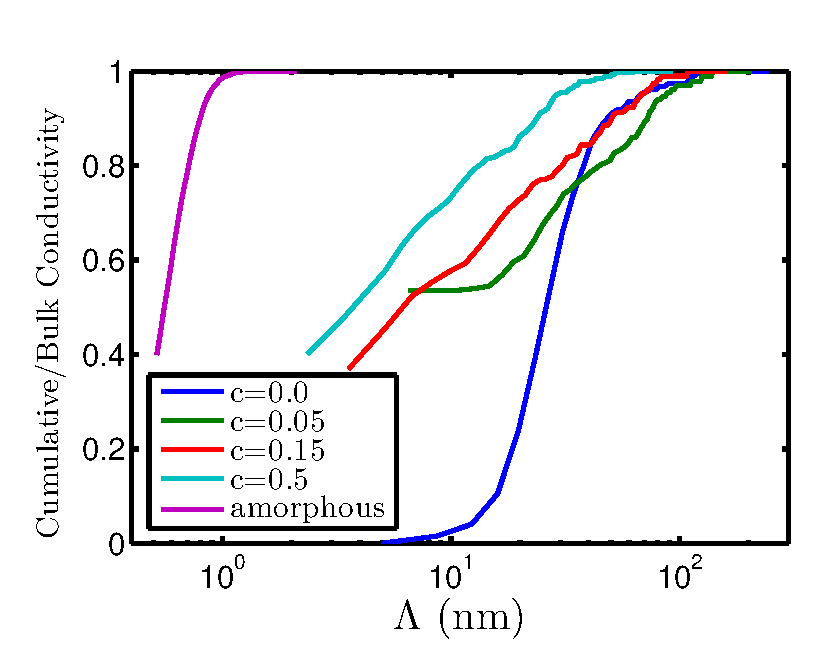
\includegraphics[scale=0.6]
{/home/jason/disorder/lj/alloy/xcorr_alloy_cum_cond.eps}
\vspace*{-5mm}
\end{center}
\caption{\label{FIG:phonon_diff} plot comparison of phonon diffusivity 
versus AF mode diffusivity for a 256 atom LJ crystal and amorphous system. 
For both systems, the total number of vibrational modes is the same.}
\end{figure}
%--------------------------------------------------------------------------

\vspace*{100mm}

%--------------------------------------------------------------------------
\subsection{\label{S:Lifetimes:}Ioffe-Regel Limit}
%--------------------------------------------------------------------------

%--------------------------------------------------------------------------
\begin{figure}
\begin{center}
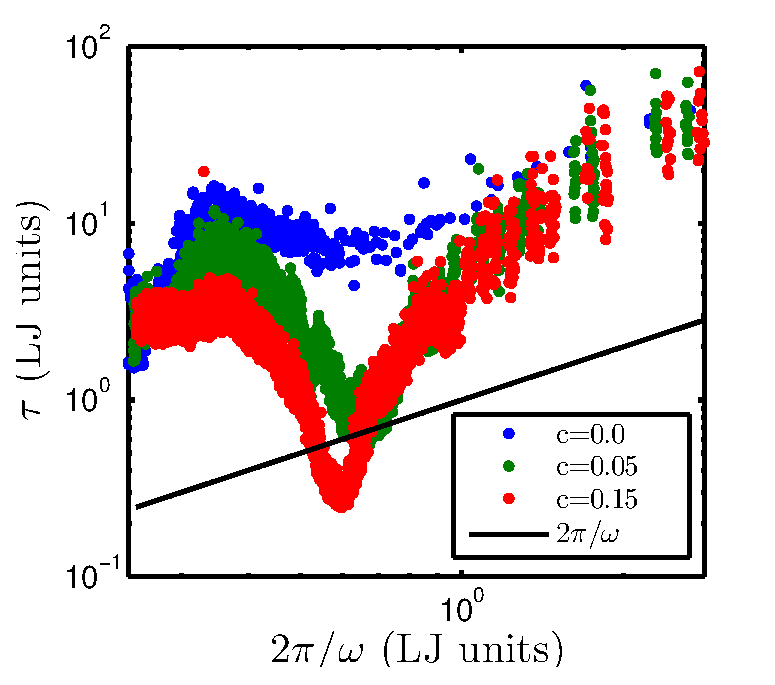
\includegraphics[scale=0.6]
{/home/jason/disorder/lj/alloy/LJ_alloy_life_period.eps}
\vspace*{-5mm}
\end{center}
\caption{\label{FIG:phonon_diff} film thickness dependant thermal 
conductivity of a-Si from experiment.}
\end{figure}
%--------------------------------------------------------------------------

%--------------------------------------------------------------------------
\begin{figure}
\begin{center}
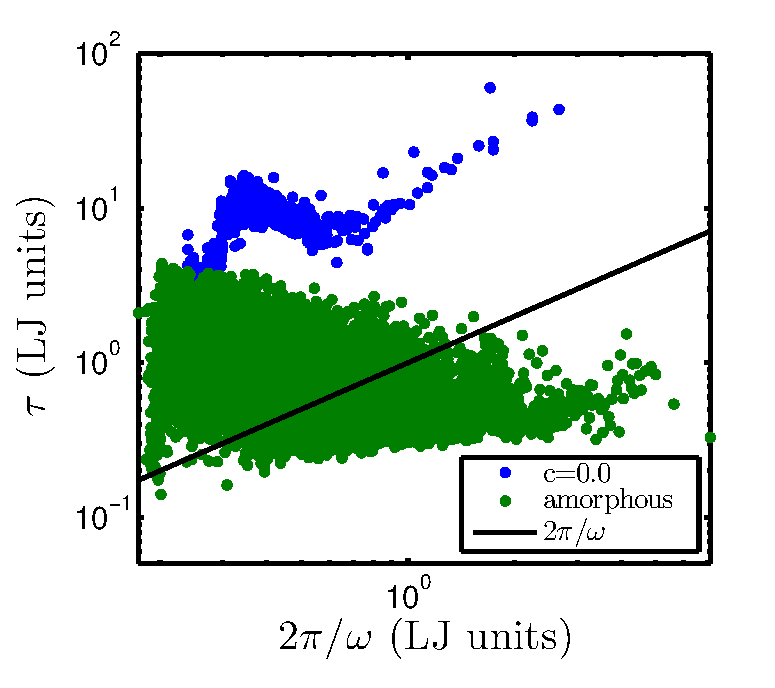
\includegraphics[scale=0.6]
{/home/jason/disorder/lj/alloy/LJ_alloy_amorphous_life_period.eps}
\vspace*{-5mm}
\end{center}
\caption{\label{FIG:phonon_diff} film thickness dependant thermal 
conductivity of a-Si from experiment.}
\end{figure}
%--------------------------------------------------------------------------

\vspace*{100mm}

%--------------------------------------------------------------------------
\subsection{\label{S:Lifetimes:}Characterization of Vibrational Modes}
%--------------------------------------------------------------------------
If determined by the Ioffe-Regel limit, $\tau \kv < 1/\omega \kv$.
\cite{taraskin_determination_1999} However, for thermal transport 
analysis this definition is not useful on its own. Show that Anderson 
loclization is exponetial depenance of mode excitation on distance from 
some local center\cite{feldman_numerical_1999}.

According to Cahill, the lifetimes of vibrations in amorphous materials 
is taken to be one half the period, $\tau = \pi/\omega $.
\cite{cahill_heat_1989}

Participation ratio:
For a finite system, the participation is limited by system size.
evolution of a vibrational wave packet on a disordered chain.
\cite{allen_evolution_1998}, shows participation ratio limitation. Also 
\cite{garber_numerical_2001}.

%--------------------------------------------------------------------------
\section{\label{S:GroupVeloctiy}Effective Mode Velocity}
%--------------------------------------------------------------------------

%--------------------------------------------------------------------------
\subsection{\label{S-Motivation-Amorphous}AF Velocity}
%--------------------------------------------------------------------------
- measured using NMD and anharmonic MD.
- extract effective Diffuson velocity, compare to sound speed

%--------------------------------------------------------------------------
\begin{figure}
\begin{center}
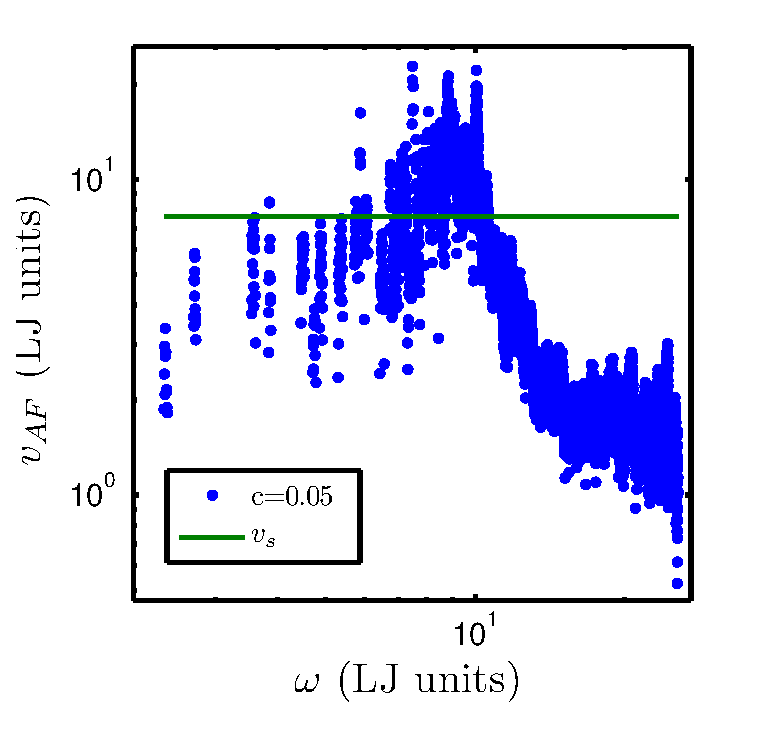
\includegraphics[scale=0.6]
{/home/jason/disorder/lj/alloy/LJ_alloy_vaf_2.eps}
\vspace*{-5mm}
\end{center}
\caption{\label{FIG:phonon_diff} AF effective velocity}
\end{figure}
%--------------------------------------------------------------------------

%--------------------------------------------------------------------------
\begin{figure}
\begin{center}
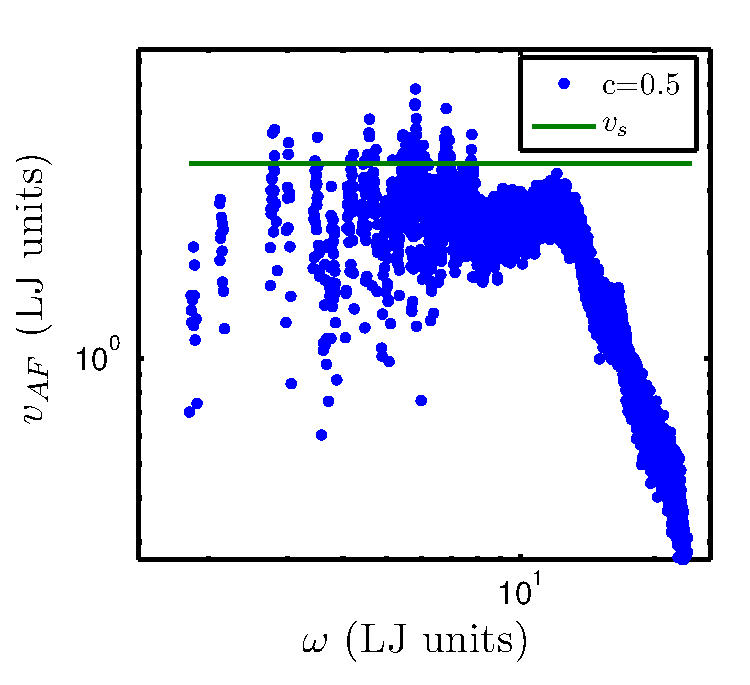
\includegraphics[scale=0.6]
{/home/jason/disorder/lj/alloy/LJ_alloy_vaf.eps}
\vspace*{-5mm}
\end{center}
\caption{\label{FIG:phonon_diff} AF effective velocity}
\end{figure}
%--------------------------------------------------------------------------

\vspace*{100mm}

%--------------------------------------------------------------------------
\subsection{\label{S:Lifetimes:}Dynamic Structrue Factor}
%--------------------------------------------------------------------------
If all modes are summed over, this gives the frequency spectrum
needed to construct a (nonstationary) propagating state with a
pure wave vector Q and pure longitudinal or transverse polarization
 \cite{feldman_thermal_1993}. Locations of spectral peaks are peaked 
like a acoustic dispersion branches. Only low-frequency vibrations 
have an (approximate) wavevector in disordered systems, and there is 
no theorem guranteeing this. \cite{feldman_numerical_1999}

However, it is very
difficult to distinguish between localized and extended
modes at high frequencies on the basis of their $S(k,\nu)$
functions, as illustrated by the very similar scattering
functions for a 67-meV localized and a 63-meV extended
mode in Fig. 3(b). \cite{biswas_vibrational_1988}

The dynamic structure factor can be useful for demonstrating the 
plane-wave character of low-frequency vibrations.  However, on a 
mode-by-mode basis, it is unable in general to characterize a given mode 
as either localized or delocalized.  In fact, results   
frequency modes in a disordered systems

%--------------------------------------------------------------------------
\begin{figure}
\begin{center}
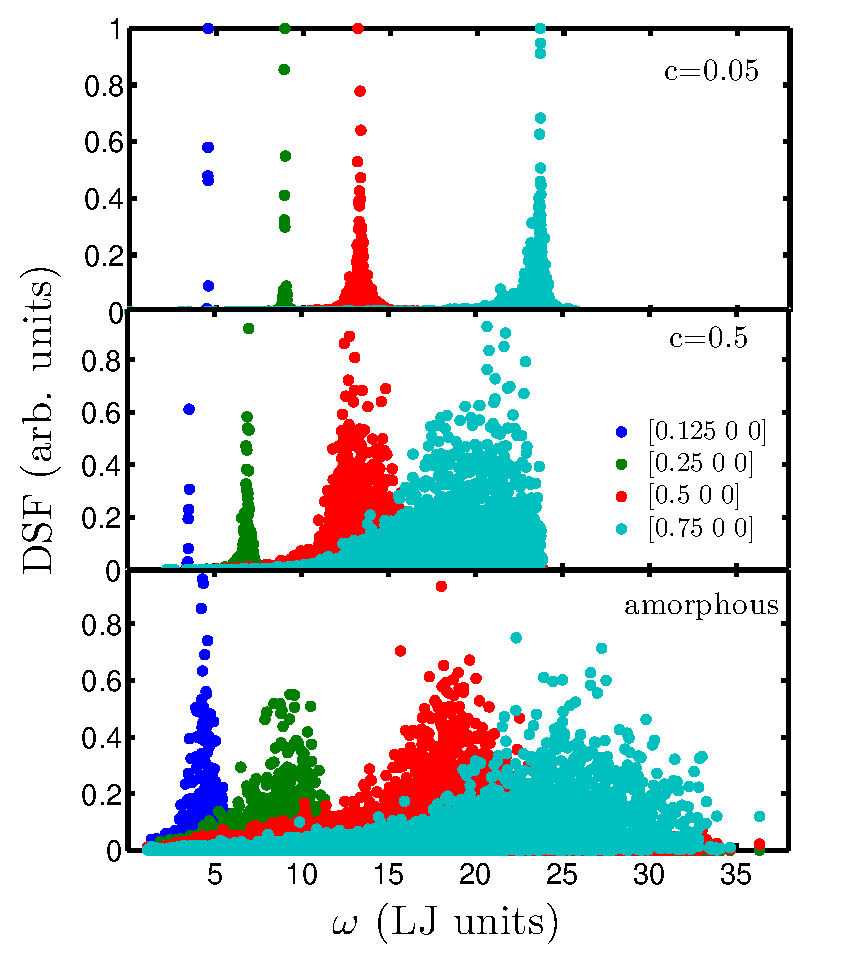
\includegraphics[scale=0.6]
{/home/jason/disorder/matlab/LJ_DSF.eps}
\vspace*{-5mm}
\end{center}
\caption{\label{FIG:phonon_diff} dynamic structure factor for LJ alloys 
and amorphous solids.}
\end{figure}
%--------------------------------------------------------------------------

\vspace*{100mm}

%--------------------------------------------------------------------------
\section{\label{S-Motivation-Amorphous}Role of Anharmonicity in 
Disordered Thermal Transport}
%--------------------------------------------------------------------------
- run harmoninc FC MD, predict thermal conductivity using GK

- compare anharmonic GK, harmonic GK, and AF predictions. May possibly 
need to run "stiffer" system to compare with 
$k_{si} = k_{ph} + k{AF} = 0.5+0.5$. 


\vspace*{100mm}


%--------------------------------------------------------------------------
\appendix
%--------------------------------------------------------------------------
\section{\label{A-Predicting-Phonons}Predicting Vibrational Lifetimes}
%--------------------------------------------------------------------------


\subsection{\label{A-Phonon-Normal-Modes}Vibrations in Ordered and 
Disordered Solids}
%--------------------------------------------------------------------------
In a crystal (periodic) system, the vibrations of atoms are described by a 
basis of eigenfunctions called phonon normal modes, which are determined by 
the properties of the crystal (see Appendix 
\ref{A-Allowed-Wavevectors-Ordered}). The eigenvalues of this basis are the 
phonon mode frequencies (energies).\cite{dove1993,wallace1972} The atomic 
velocities can be represented by the velocity normal mode coordinate, 
defined as 
\cite{dove1993}
\begin{equation}\label{E:udot_HLD}
\begin{split}
\dot{u}_{\alpha}\lbt = &\SUMprime{2}{} \frac{1}{\sqrt{m_bN}} 
\EXP{i\pmb{\kappa}^{'}\cdot\mathbf{r}_0\ab{l}{0}} e^*\kvba 
\dot{q}\kvt{}{}{}.
\end{split}
\end{equation}
Here, $\dot{q}\kvt{}{}{}$ represents the kinetic energy $T \kvt$ of the 
mode with phonon frequency $\omega_0\kv$ by
\cite{dove1993}
\begin{equation}\label{E:udot_HLD}
\begin{split}
T \kvt= \frac{\dot{q}^*\kvt{}{}{}\dot{q}\kvt{}{}{}}{2}.
\end{split}
\end{equation}
The phonon mode kinetic energies $T \kvt$ are used to calculate the phonon 
spectral energy denisty in Appendix \ref{A-Phonon-Life-SED}.

\subsection{\label{A-Allowed-Wavevectors-Ordered}Allowed Wavevectors in 
Ordered Systems}
%--------------------------------------------------------------------------
The phonon spectral energy is defined for the allowed wavevectors of a 
crystal, which can be specified from the crystal structure's Bravais 
lattice and its basis, i.e. unit cell. A $D$-dimensional Bravais lattice 
is a collection of points with
positions
\begin{equation}\label{crys_pos}
\begin{split}
\mathbf{u}_0\ab{l}{0} =& \sum^D_{\alpha} N_{\alpha}\mathbf{a}_{\alpha}
\end{split}
\end{equation}
where $N_{\alpha}$ and the summations if over the lattice vectors, 
$\mathbf{a}_{\alpha}$.\cite{ashcroft1976} The basis (or unit cell) is the 
building block of the crystal and they are arranged on the points defined 
by the Bravais lattice. The equillibrium position of any atom in the crystal 
can be described by
\begin{equation}\label{crys_pos2}
\begin{split}
\mathbf{u}_0\ab{l}{b} = \mathbf{u}_0\ab{l}{0} + \mathbf{u}_0\ab{0}{b}
\end{split}
\end{equation}
where $\mathbf{u}_0\ab{l}{0}$ is the equilibrium position of the 
$l^{\textrm{th}}$ unit cell and $\mathbf{u}_0\ab{0}{b}$ is the equilibrium 
position of the and $b^{\textrm{th}}$ atom in the unit cell relative to 
$\mathbf{u}_0\ab{l}{0}$.
For the LJ systems studied here, the cubic conventional cells are used with 
four atoms per unit cell.\cite{ashcroft1976} For our MD simulations, cubic 
simulation domains with periodic boundary conditions are used with 
$N_1 = N_2 = N_3 = N_0$.\cite{turney2009a,mcgaughey2004a} The allowed 
wavevectors for such crystal structures are
\begin{equation}\label{crys_pos3}
\begin{split}
\pmb{\kappa} = \sum_{\alpha} \mathbf{b}_{\alpha} 
\frac{n_{\alpha}}{N_{\alpha}},
\end{split}
\end{equation}
where $\mathbf{b}_{\alpha}$ are the reciprocal lattice 
vectors\cite{ashcroft1976} and $-N_{\alpha}/2 < n_{\alpha} 
\leq N_{\alpha}/2$, where $n_{\alpha}$ are integers and $N_{\alpha}$ 
are even integers.\cite{turney2009a} The wavevectors are taken to be 
in the first Brioullin zone.\cite{ashcroft1976}

%--------------------------------------------------------------------------
\subsubsection*{Allowed Wavevectors in Disordered Materials}
%--------------------------------------------------------------------------
Strictly speaking, the only allowed wavector in a disordered system is the 
gamma point ($\kappa = [0 0 0]$). As such, the lattice dynamics calculations 
are performed at the gamma point:


%--------------------------------------------------------------------------
\subsection{\label{S:Lifetimes:}Normal Mode Decomposition}
%--------------------------------------------------------------------------
Normal mode decomposition and its limitations.
\cite{turney_predicting_2009-1} 

If $\gamma \kv > \omega \kv$, then the vibrational mode is overdamped.  
Discuss why real-space method is necessary in this case.


%--------------------------------------------------------------------------
\subsection{\label{A-Thermal-Cond}Thermal Conductivity}
%--------------------------------------------------------------------------
Once the lifetimes (MFPs) and group velocities of all virbrational modes 
in the
Brillouin zone are obtained, the bulk thermal conductivity in direction
$\mathbf{n}$, $k_{\mathbf{n}}$, can be calculated from \cite{ziman2001}
\begin{equation}\label{E-size:k_bulk}\
\begin{split}
k_{\mathbf{n}}=&\sum_{\pmb{\kappa}} \sum_\nu c_{ph} \kv v^{2}_{g,\mathbf{n}} 
\kv \tau \kv.
\end{split}
\end{equation}
Here, $c_{ph}$ is the phonon volumetric specific heat and 
${v}_{g,\mathbf{n}}$ is
the component of the group velocity vector in direction $\mathbf{n}$. 
Since the systems we consider are classical and obey Maxwell-Boltzmann 
statistics,\cite{mcquarrie2000} the
specific heat is $k_{B}/V$ per mode in the harmonic limit where $V$ 
is the system volume. This approximation is used here and has been shown 
to be suitable for LJ argon\cite{mcgaughey2004c} and SW silicon.
\cite{goicochea2010} The group
velocity vector is the gradient of the dispersion curves 
(i.e., $\partial \omega / \partial \pmb{\kappa}$), which can be 
calculated from the frequencies and wavevectors using finite differences. 
In this work, the group velocities are calculated using finite difference 
and quasi-harmonic lattice dynamics because a very small finite difference 
can be used which reduces the error.\cite{mcgaughey2006b} To predict a 
bulk thermal conductivity, it is necessary to perform a finite simulation 
size scaling procedure as discussed in Appendix \ref{A-Finite-Sim}.

%--------------------------------------------------------------------------
\section{\label{A-Finite-Sim}Finite Simulation-Size Scaling for Thermal 
Conductivity}
%--------------------------------------------------------------------------
For the LJ argon system studied in Section \ref{S-Prelim-Vib-Cond-Ordered}, 
a finite simulation-size scaling procedure\cite{turney2009a,He2011a} is 
used to compare the thermal conductivity predictions from $\Phi$ and $\Phi'$ 
to those from the Green-Kubo method. The scaling procedure is demonstrated in 
Fig$.$ \ref{FIG:LJ_COND}. The thermal conductivity is predicted from $\Phi$ 
or $\Phi'$ and MD simulations with $N_0 = 4,6,8,$ and $10$. The bulk 
conductivity, $k_{\infty}$, is then estimated by fitting the data to
\begin{equation}\label{k_size}
\begin{split}
1/k = 1/k_{\infty} + A/N_0,
\end{split}
\end{equation}
where $A$ is a constant. This procedure is necessary because the first 
Brillouin zone is only sampled at a finite number of points for a finite 
simulation size, with no contribution from the volume at its center. To 
predict a bulk thermal conductivity, it is important to sample points near 
the Brillouin zone center, where the modes can have large lifetimes and 
group velocities.\cite{turney2009a,sellan2010b} 
%--------------------------------------------------------------------------
\begin{figure}
\begin{center}
%\includegraphics[angle=0,width=70.0mm]{LJ_NMD_SED_COND_2.eps}
\end{center}
\caption{\label{FIG:LJ_COND} Thermal conductivity predictions for LJ argon calculated using phonon lifetimes predicted by $\Phi$ and $\Phi'$.\cite{Larkin2012} (a) The finite simulation-size scaling extrapolation \cite{turney2009a,He2011a} is used to compare the results to bulk predictions made using the Green-Kubo method. (b) The bulk results for $\Phi$ and Green-Kubo are in good agreement temperatures of $20$ and $40$ K with those of other atomistic simulation methods.\cite{turney2009a}}
\end{figure}
%--------------------------------------------------------------------------


\clearpage
\bibliographystyle{apsrev}
\bibliography{/home/jason/ntpl-ref/ntpl-jason/ntpl-jason-091712}
\end{document}
